% Template for a Thesis
%
% 6-results.tex
%
% Results

\chapter{Results}\label{ch:results}

\section{Replication of BPE}

The results show that BPE increases word alignment results, specifically the F1 score is increased by 0.5\% on average for different number of symbols, the most notable improvement being with 1000 BPE symbols, and a F1 score improvement of 0.9\%.

\begin{figure}[!ht]
    \centering
    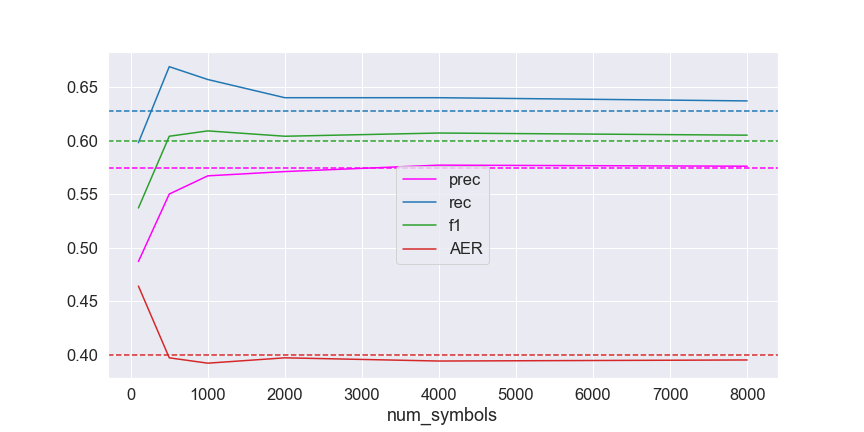
\includegraphics[width=14cm]{figures/eng_deu_fastalign.png}
    \caption{Scores of BPE over baseline}
\end{figure}

\section{Replication of BPE dropout}

In order to make a comparison between BPE and BPE dropout, the BPE scores are taken as baseline, instead of the gold standard's scores as in the previous case.

%\begin{figure}[!ht]
%    \centering
%    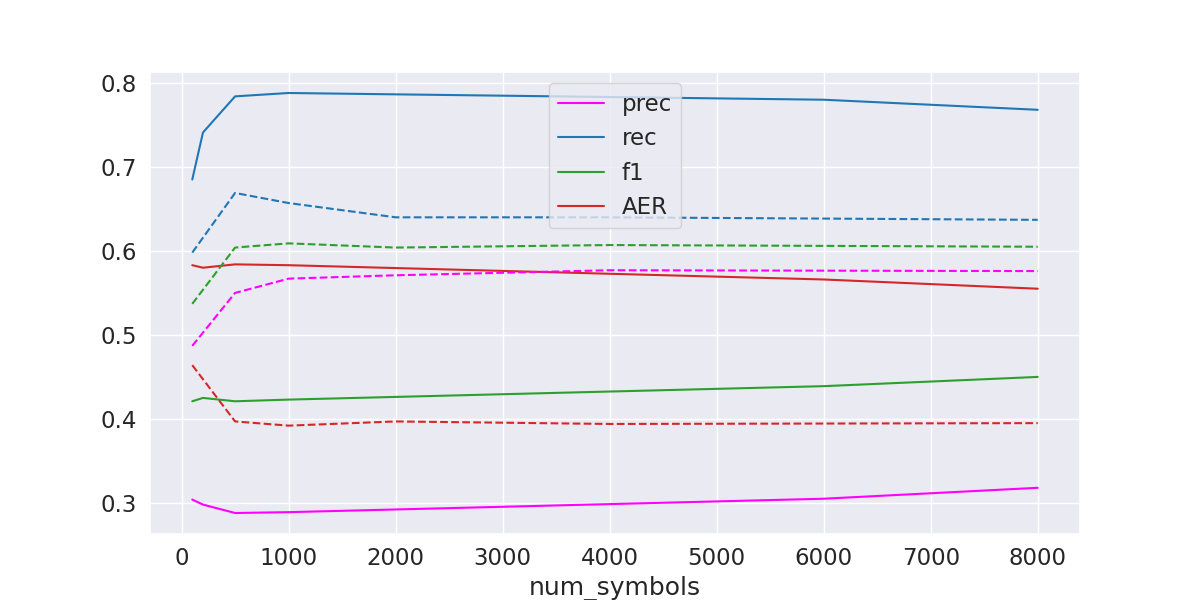
\includegraphics[width=14cm]{../reports/scores_dropout_bpe/space/0.1/union_fastalign.png}
%    \caption{Scores for BPE with dropout 0.1, union mode}
%\end{figure}
%
%\begin{figure}[!ht]
%    \centering
%    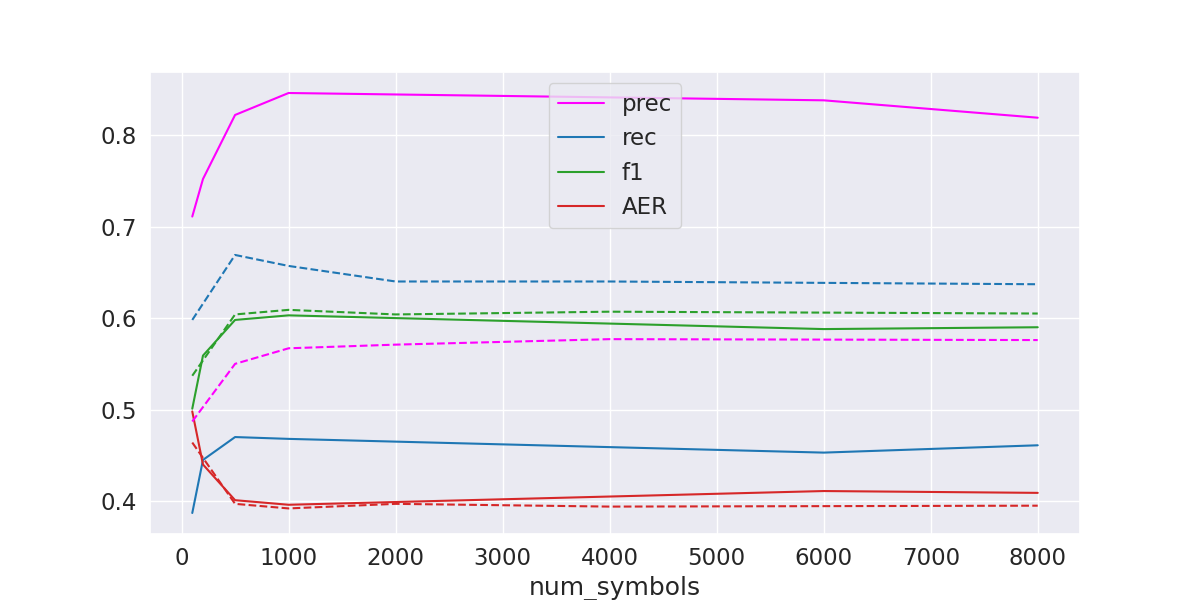
\includegraphics[width=14cm]{../reports/scores_dropout_bpe/space/0.1/inter_fastalign.png}
%    \caption{Scores for BPE with dropout 0.1, inter mode}
%\end{figure}

As mentioned above, the union scores have a very high recall compared to the BPE scores, and the intersection score has much better precision. Various threshold values have been computed, namely 0.3, 0.5, 0.7 and 0.9. For the sake of brevity, the one with the best score is shown, which is when the threshold is 0.7.

%\begin{figure}[!ht]
%    \centering
%    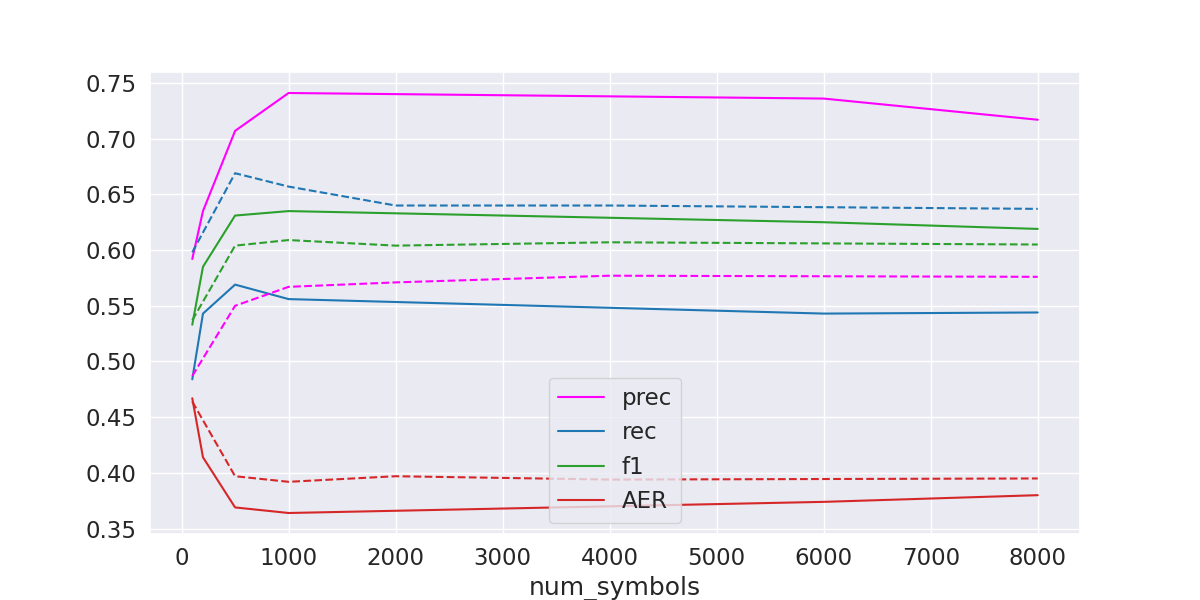
\includegraphics[width=14cm]{../reports/scores_dropout_bpe/space/0.1/0.7_thres_fastalign.png}
%    \caption{Scores for BPE with dropout 0.1, threshold mode at 0.7}
%\end{figure}

As the BPE dropout paper states~\cite{provilkov2019bpedropout}, BPE dropout improves BPE consistently no matter how many num\_symbols are employed.

